% !TeX spellcheck = en_US
% !TeX encoding = UTF-8 

\documentclass[14pt,a4paper]{extarticle}

\usepackage[english]{babel}
\usepackage[utf8]{inputenc}
\usepackage{setspace} 
\usepackage[a4paper,
	left=30mm,
	right=10mm,
	top=20mm,
	bottom=20mm]{geometry}
\usepackage{amsmath}
\usepackage{amssymb}
\usepackage{amsthm}
\usepackage{graphicx} 
\usepackage{cite}
\usepackage{subfigure}
\usepackage{subcaption}
\usepackage{kprjHSE} 
\usepackage{listings}
\usepackage{tabu}
\usepackage{courier}

\lstset{
	frame=single,
	basicstyle=\ttfamily,
	breaklines=true,
	tabsize=4
}

\LabWork
\LabWorkNo{2}

\FirstAuthor{M.D.~Kirdin}
\FirstConsultant{A.~Tomat}
\SecondConsultant{M.~Zueva}
\discipline{Ordered Sets for Data Analysis}
\faculty{Faculty of Computer Science}
\chair{School of Data Analysis and Artificial Intelligence}
\chief{S.O.~Kuznetsov}
\workyear{2024}

\onehalfspacing

\begin{document}
	\maketitle
	
	\subsection*{Question 1}
	\noindent\textbf{Task.} Given the following formal context, find all formal concepts, draw the concept lattice,
	and find all non-trivial implications.
	\begin{center}
	\begin{tabu}{ |X[c]|X[c]|X[c]|X[c]|X[c]|X[c]|}
		\hline
		 & a & b & c & d & e\\
		\hline
		1 & 1 &  & 1 &  & 1\\
		\hline
		2 & 1 &  & 1 & 1 & \\
		\hline
		3 & 1 &  &  & 1 & 1\\
		\hline
		4 & 1 & 1 &  & 1 & \\
		\hline
		5 & 1 & 1 &  &  & 1\\
		\hline
	\end{tabu}
	\end{center}
	 
	 \noindent\textbf{Solution.}
	 
	 
	 \begin{figure}[h]
	 	\centering
	 	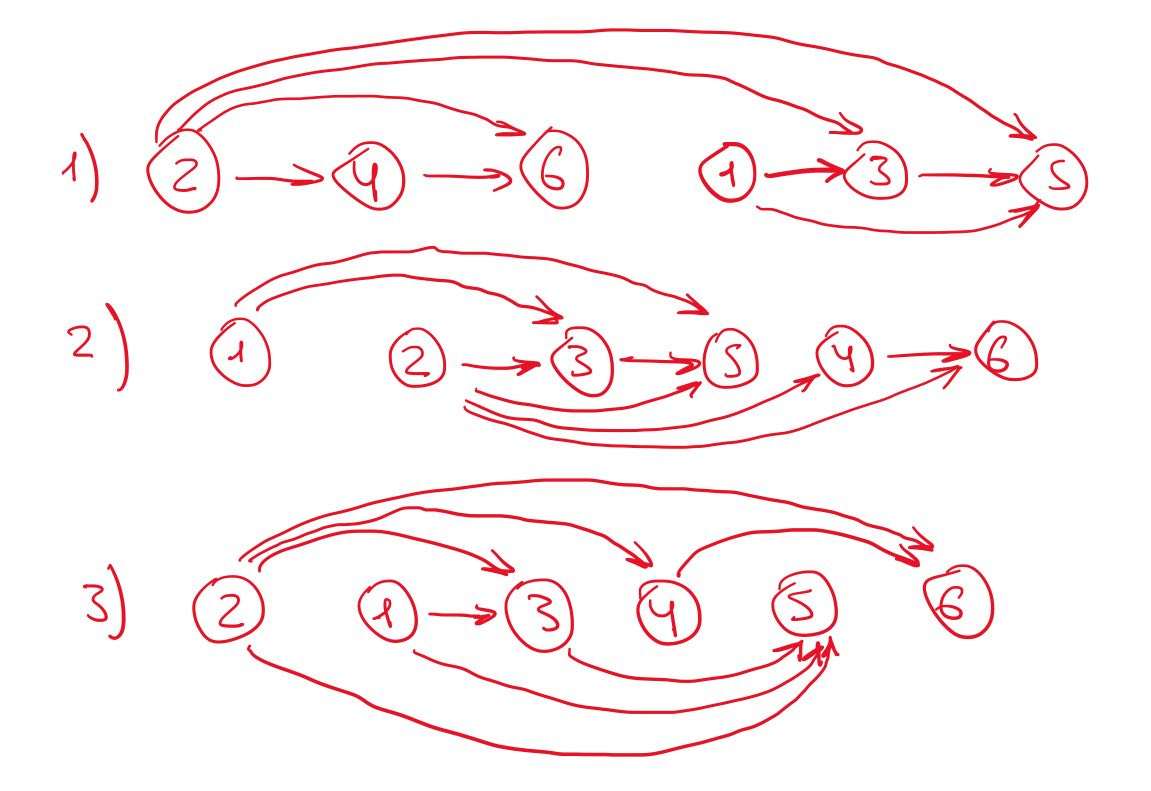
\includegraphics[scale=0.3]{media/toposort.jpg}
	 	\caption{Three different topological sorts for the graph on \figref{fig:graph}}
	 	\label{fig:toposort}
	 \end{figure}
	 
\end{document}